% Nome do capítulo
\chapter{Conclusões e Trabalhos Futuros}
% Label para referenciar
\label{ch:conclusao}

% Diminuir espaçamento entre título e texto
\vspace{-1.9cm}
O objetivo geral de se aprimorar a luva de \citeonline{roversi} para captura dos movimentos de adução e abdução foi atingido, mas os resultados não foram totalmente satisfatórios, já que os sensores não conseguiram captar movimentos pequenos dos dedos, devido às limitações dos sensores e do \textit{Arduino} e, a movimentação do dedo médio não foi captada devido à necessidade de uma referência fixa para obter os ângulos de dobra entre os dedos.

A captação dos movimentos de desvio radial e ulnar do pulso foi atingida, oferecendo movimentos fluidos e, apesar da posição do \textit{Arduino} limitar alguns movimentos, o método se mostrou preciso.

A redução de ruídos dos sensores também foi atingida, fornecendo boa redução de ruídos e mantendo a responsividade.

A correção das falhas de \textit{hardware} do trabalho de \citeonline{roversi} foi atingida construindo um novo circuito em um \textit{shield} de prototipagem com um conector de barra para permitir a remoção dos sensores e melhorar as conexões entre os componentes.

Os requisitos de \textit{hardware} propostos  foram parcialmente atingidos, pois alguns componentes da luva, como o tecido e o \textit{Arduino}, ainda limitaram movimentos como os de extensão do pulso e de abdução do polegar

Os requisitos de \textit{software} foram atingidos parcialmente, pois a amplitude dos movimentos reais diferiu dos movimentos reproduzidos pelo modelo e os movimentos dos dedos foram prejudicados pela baixa resolução dos sensores de flexão. Por outro lado, a reprodução da orientação da mão foi satisfatória, com resultados precisos e movimentos fluidos.

O custo total dos componentes da luva foi de R\$ 982,69 e os preços de cada componente são apresentados na Tabela \ref{tab:custos}.

\begin{table}[H]
  \centering
  \footnotesize
  \setlength{\abovecaptionskip}{0pt}
  \setlength{\belowcaptionskip}{0pt}
  \caption[Custo do Projeto]{Custo do Projeto}
  \label{tab:custos}
  \begin{tabular}{l r}
    \hline\hline
    \multicolumn{1}{c}{Componentes}&\multicolumn{1}{c}{Preço Total}\\
    \hline
    01 $\times$ \textit{Arduino Mega}                                 & R\$ 59,00 \\
    02 $\times$ \textit{MPU-9250}                                     & R\$ 84,00 \\
    02 $\times$ Conectores em barra de 40 pinos                       & R\$ 3,00 \\
    01 $\times$ \textit{Shield} de Prototipagem para \textit{Arduino} & R\$ 29,90 \\
    14 $\times$ Sensores de flexão                                    & R\$ 728,00 \\
    14 $\times$ Resistores (\SI{10}{\kilo\ohm})                       & R\$ 1,40 \\
    40 $\times$ Fios \textit{jumper}                                  & R\$ 13,80 \\
    01 $\times$ Tubo Termo Retrátil                                   & R\$ 1,60 \\
    01 $\times$ Par de luvas de neoprene                              & R\$ 49,99 \\
    01 $\times$ Par de luvas de \textit{lycra}                        & R\$ 12,00 \\
    \hline
    Total                                                             & R\$ 982,69 \\
    \hline\hline
  \end{tabular}
  \\\vspace{1.3mm}
  \captionfont{\small{\textbf{Fonte: Elaborado pelo Autor}}}
\end{table}

\section{Trabalhos Futuros} % (fold)
\label{sec:trabFut}
Os possíveis trabalhos futuros para melhoria deste projeto incluem a utilização de uma luva com material diferente que facilite a sua colocação e retirada da mão, e que permita a transpiração para permitir o uso por períodos prolongados. 

Além disso é necessário uma melhor fixação do \textit{Arduino} no braço do usuário, ou ainda uma solução que capture os movimentos sem a necessidade do \textit{Arduino} preso ao usuário, para possibilitar a liberdade de movimentos. Também seria importante que a transmissão de dados para o computador fosse feita por \textit{Bluetooth} ou \textit{Wi-Fi}, eliminando assim a necessidade de fios e cabos que podem atrapalhar os movimentos.

Para melhorar a sensibilidade dos sensores, poderiam ser analisados algoritmos tais como o filtro de Kalman ou a técnica de suavização exponencial com diferentes parâmetros de sensibilidade, para reduzir o impacto dos ruídos e suavizar os movimentos.

Seria ideal para aplicações médicas ou de \ac{RV} uma solução que captasse os movimentos menores e mais complexos dos dedos e da mão, como por exemplo o movimento de abrir ou fechar a palma da mão (oposição e reposição) mostrado na Figura \ref{fig:oprep}, fazendo uso de sensores com mais resolução em relação aos que foram utilizados neste trabalho, ou implementando uma solução melhor para suavização das leituras dos sensores. Uma alternativa seria utilizar transdutores lineares ópticos, como no projeto de \citeonline{li2009smartglove}, que forneceriam leituras mais estáveis para os movimentos de flexão e extensão.

\begin{figure}[H]
  \setlength{\abovecaptionskip}{0pt}
  \setlength{\belowcaptionskip}{0pt}
  \caption[Movimentos de Oposição e Reposição]{Movimentos de Oposição e Reposição}
  \centering
  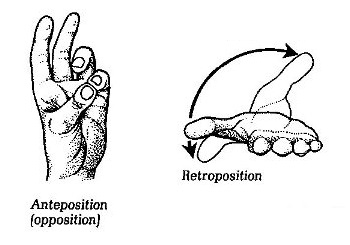
\includegraphics[width=.5\textwidth]{imagem/thumb-workings.jpg}
  \captionsetup{justification=centering}
  \captionfont{\small{\textbf{\\Fonte: \citeonline{movimentos}}}}
  \label{fig:oprep}
\end{figure}

Outras possíveis aplicações para esta luva incluem captura de movimentos para animações ou controle de braços robóticos à distância e reconhecimento de gestos para tradução de linguagem de sinais.

% Texto do capítulo